\section{Block Definition Diagram}
\label{sec:blockdefinitiondiagram}

Das Block Definition Diagram (siehe Abb. \ref{fig:block1}) in dieser Phase stellt den groben, physikalischen Aufbau der \textit{Smartwatch} dar. Diese setzt sich zusammen aus \textit{Sensoren}, einem \textit{Display}, einem \textit{Speichermedium}, einem \textit{Armband}, einen \textit{Gyroskop}, einer \textit{Bluetooth-Antenne} und einem \textit{GPS-Modul}. Um die Stromversorgung der Uhr zu garantieren, soll das \textit{Armband} aus mehreren \textit{Akkuzellen} bestehen. Das \textit{Display} soll dabei komplett von dem \textit{Armband} trennbar sein. So kann die Uhr bei schwachen Akku oder bei einem Wechsel zu einer sportlichen Tätigkeit einfach in einem anderen \textit{Armband} eingesetzt werden. Für die Smartwatch wird das \textit{Gewicht in Gramm}, die \textit{Abmessungen in Millimetern} und die \textit{Auflösung des Displays in Zoll} angegeben. Für das \textit{Armband} wird das \textit{Gewicht in Gramm}, der \textit{Umfang des Bandes in Zentimetern} und die \textit{Farbe} angegeben. Die Akkuleistung wird in Watt beschrieben. Die \textit{Bluetooth-Antenne} soll die Verbindungsstelle zum \textit{Smartphone} sein. Um die Akkulaufzeit zu erhöhen soll die \textit{Antenne}, zusätzlich zum normalen Bluetooth, auch \textit{"Low-Energy" -Bluetooth} unterstützen. Die Smartwatch selbst soll keine Daten, außer die für die Nutzung reiner Sportaktivitäten benötigten, speichern können. Daher ist der \textit{Speicher} recht klein gehalten und dient nicht zum verwalten von Bildern oder anderen Benutzerdaten.
Zu diesem Zeitpunkt der Entwicklung waren die Funktionalitäten noch nicht fertig festgelegt und deshalb fehlen im Diagramm unter anderem die Tasten für das Skalieren und Weiterblättern des Bildschirms und eine genauere Spezifikation der Sensoren.

\begin{figure}[h]
\centering\
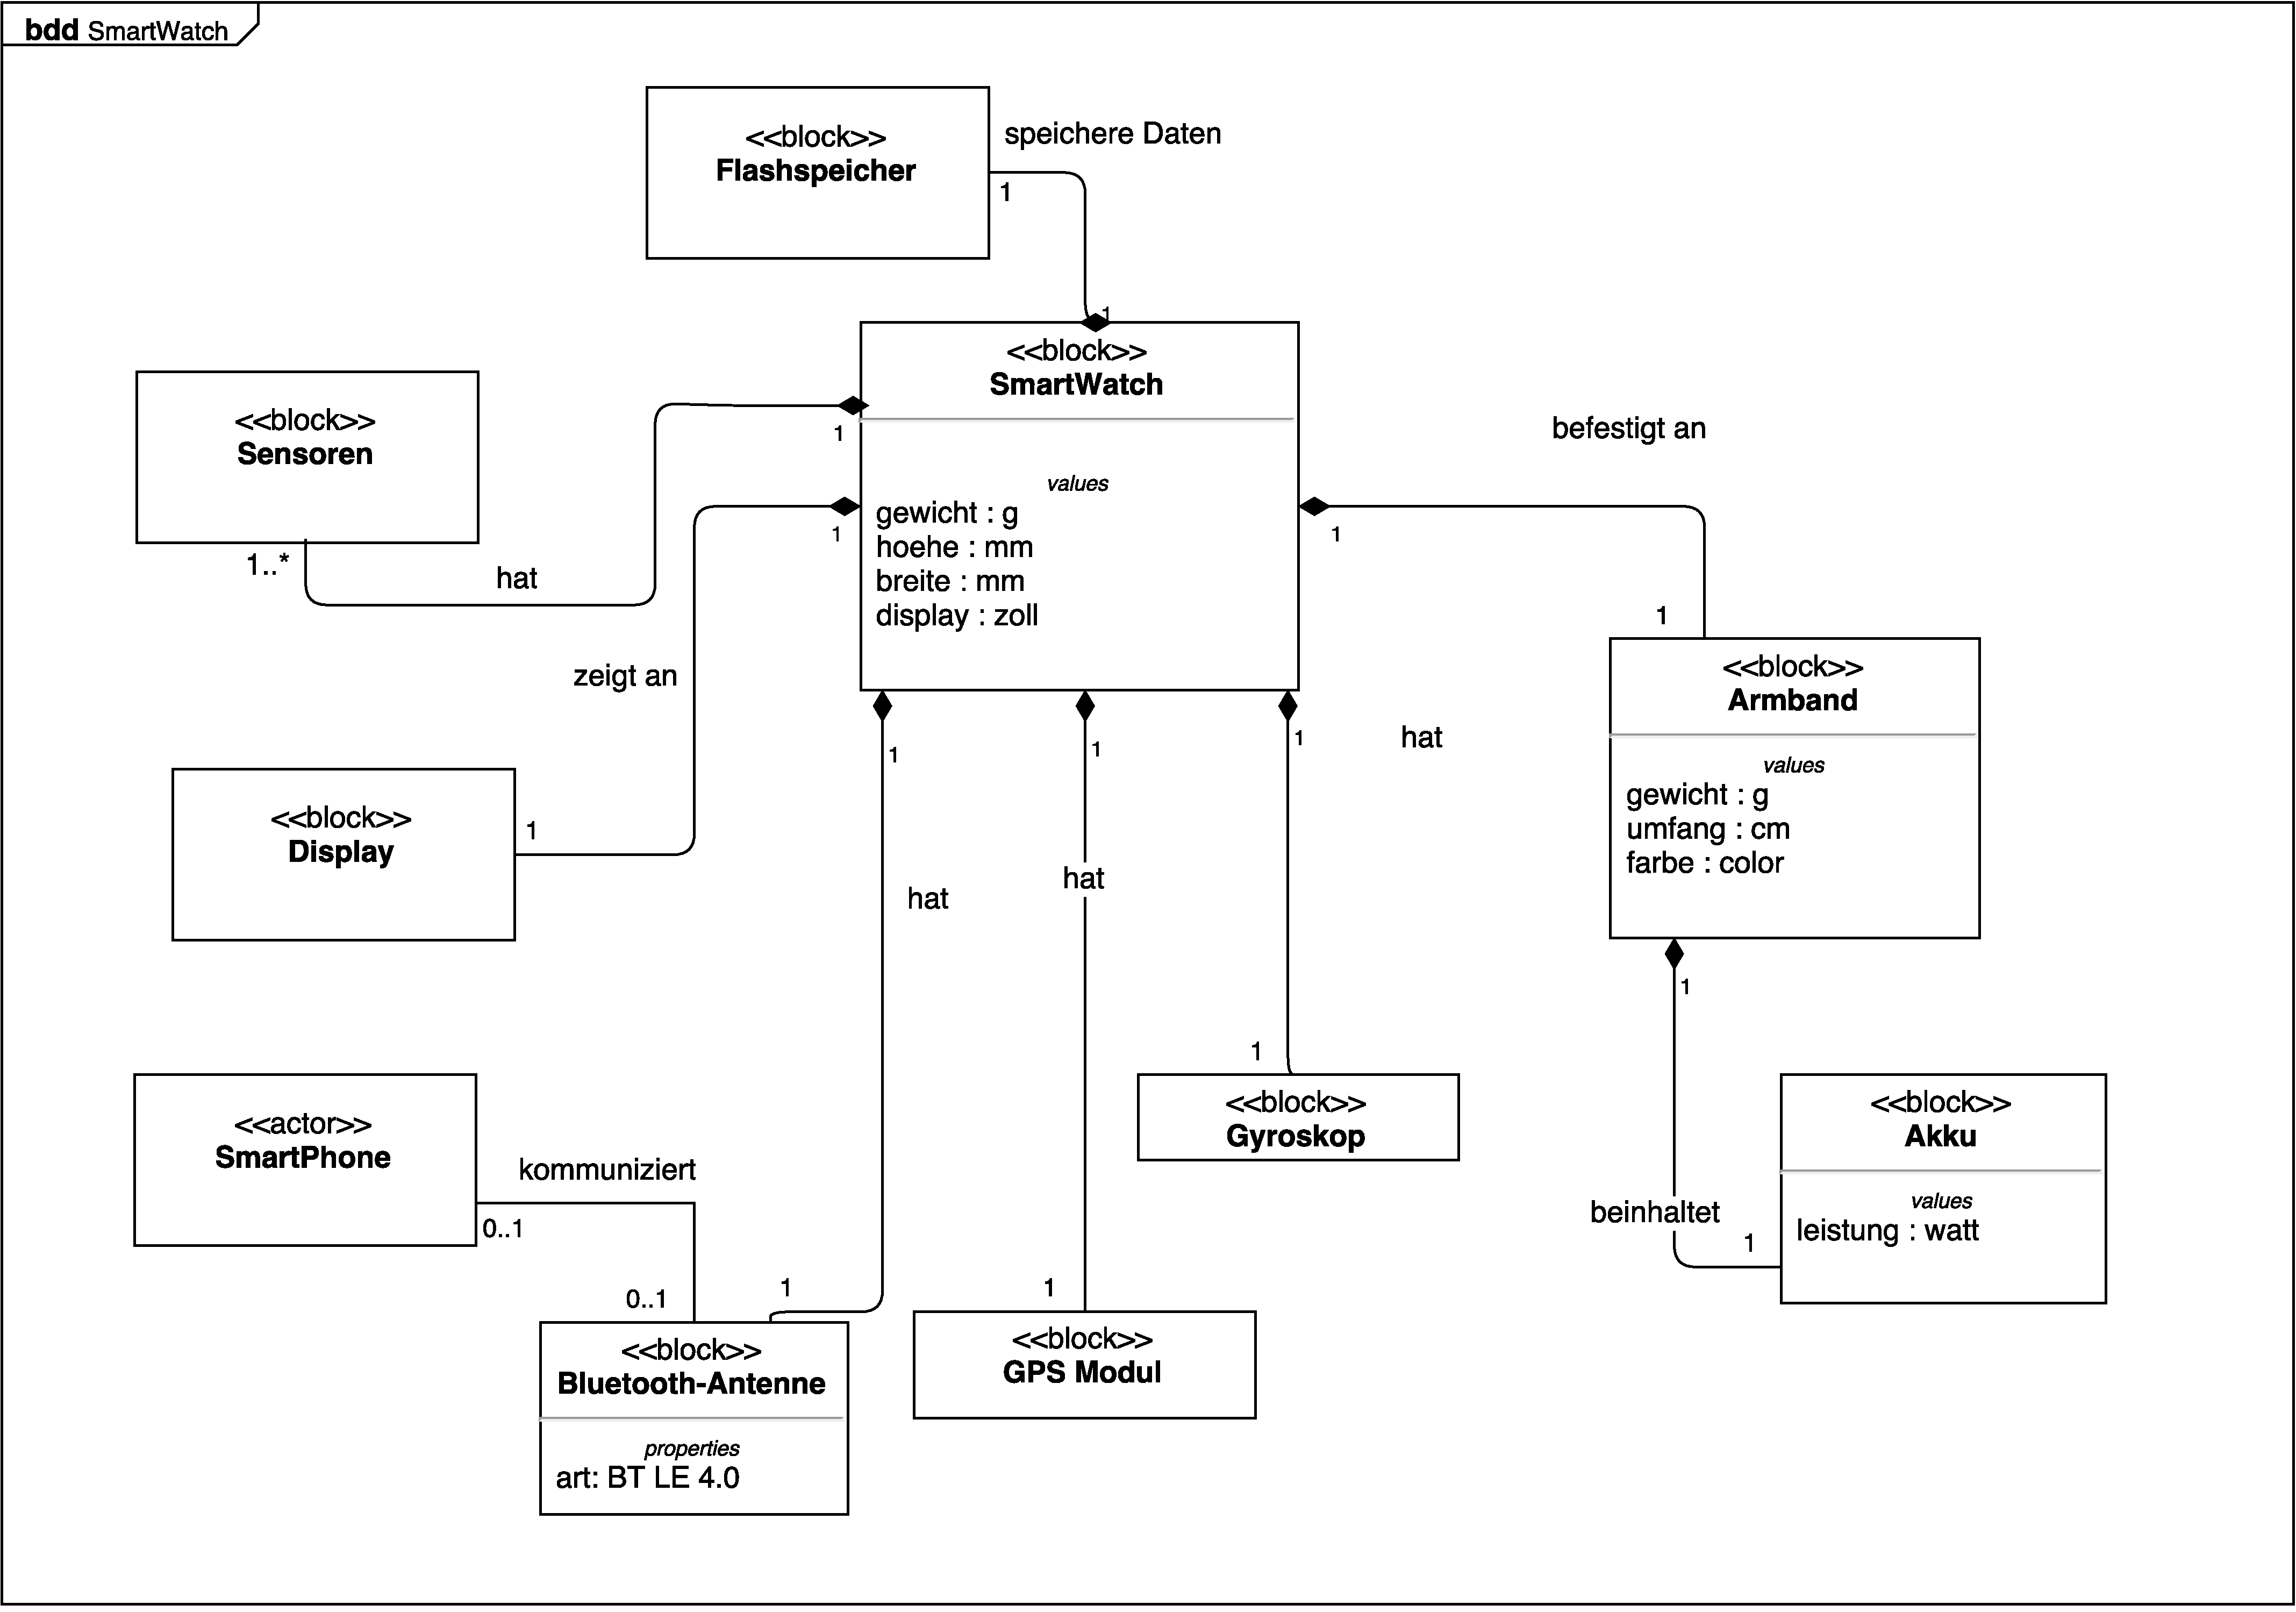
\includegraphics[width=\textwidth]{img/block1}
\caption{Erstes Blockdefinitionsdiagramm für den physikalischen Aufbau der Smartwatch.}\label{fig:block1}
\end{figure}